
\documentclass{article}
\usepackage{graphicx}
\usepackage{listings}
\usepackage{graphics}
\usepackage[T1]{fontenc}
\usepackage[margin=1.2in]{geometry}
\usepackage{tcolorbox}
\usepackage{hyperref}
\usepackage{dingbat}
\usepackage{float}
\begin{document}

\begin{titlepage}
\title{Basics of rtos}
\author{e-Yantra Team }
\date{July 2016}



\maketitle

\end{titlepage}

\listoffigures
\tableofcontents
\newpage

\section{Introduction to RTOS}
\subsection{What is RTOS ?}
"RTOS" stands for Real-Time Operating System.
It is a type of operating system used for real time applications in embedded systems.
RTOS is known for its characteristics that helps is in many applications.
\begin{itemize}

\item Reliability :\\
RTOS provides more reliability as compared to GPOS.
It has more control over events in real time and they are always available to provide service.
Some systems are required to run for a longer period of time without human intervention, for these purposes RTOS can be very useful.

\item Determinism:\\
 RTOS entirely functions over deadlines which makes            it more efficient.
It means that for each process a specifc deadline or a time-period is specified within which it has to finish that particular process.

\item Scheduling:\\
 In this operating system, user has more control over scheduling a particular task or a process depending on its priority.
So we can define the priority for that particular  task and also the frequency with which it should occur ( more like a delay).
In GPOS all the scheduling functions are process based and user has less control on them.
Task defined in RTOS are preemptive. 
Generally, in an operating systems there are two types of tasks viz. High priority tasks and Low priority tasks.
High priority task can meet their deadlines consistently because of the preemptive property.

\item Scalability:\\
RTOS is used in wide variety of applications in the field of embedded systems.
So it is scalable depending on the application requirements (i.e we can add or remove modular components depending on our use).
\end{itemize}

\subsection{Types of tasks in RTOS}
\begin{enumerate}
    

\item\textbf{Hard real-time tasks:}\\
These types of tasks strictly run based on deadlines.
If a particular task is not finished within the predetermined deadlines  then the system is considered to be a failed system.
Applications : Anti-missile systems, Air bag mechanisms etc.

\item\textbf{Firm real-time tasks:}\\
Similar  to hard real-time tasks they should also meet the deadlines.
But if they don't meet then that doesn't make this a failed system, but the results that are produced after the deadlines are discarded and the utility of the system becomes zero.
Applications : Multimedia

\item\textbf{Soft real-time systems:}\\
Here the deadlines are not expressed as some absolute value but they are expressed as a average response time required by the task.
If the task is finished then the utility of the task is 100%. But if they fail to meet them, then the utility of the system gradually falls depending on the extra time that is taken past the deadline.  
\end{enumerate}

\section{Multi-tasking}
The number of resources available in a system are limited and need to be shared across different processes/tasks. For the proper allocation of resources an operating system provides different techniques by which a user can allocate resources or restrict resources for few particular tasks.\\
\textbf {MultiTasking:}
Multitasking is running multiple processes at the same time.
In a multi-processor system it implies that each core of processor is executing different tasks i.e. multiple tasks at the same time.
Whereas in a single processor system the operating system schedules tasks in such a way that all the tasks are performed simultaneously i.e. each task gets a limited amount of Processor time, after the time expires the running task is suspended and another task is executed. The original task gets the resources again when all the tasks are given equal amount of processor time. 

\section{Semaphore}
\subsection{Semaphore}
A semaphore is a value in a designated place in operating system (or kernel) storage that each process can check and then change. Depending on the value that is found, the process can use the resource or will find that it is already in use and must wait for some period before trying again.
Semaphores basically is a variable which indicates number of units of a particular resource that are available. Each semaphore(S) has two associated functions (P, V) which can only change the value of S.
A simple way to understand \textbf{Wait (P)} and \textbf{Signal (V)} operations is:
\begin{itemize}
    
\item\textbf {Wait:}\\ 
If the value of semaphore variable is not negative, decrements it by 1. If the semaphore variable is now negative, the process executing wait is blocked (i.e., added to the semaphore's queue) until the value is greater or equal to 1. Otherwise, the process continues execution, having used a unit of the resource.
\item\textbf {Signal:}\\
Increments the value of semaphore variable by 1. After the increment, if the pre-increment value was negative (meaning there are processes waiting for a resource), it transfers a blocked process from the semaphore's waiting queue to the ready queue.
\end{itemize}
\subsection{Mutex}
Mutex is a property of concurrency control, which is instituted for the purpose of preventing race conditions; it is the requirement that one thread of execution never enter its critical section at the same time that another, concurrent thread of execution enters its own critical section.
Mutex refers to a variable that tells if a given resource is available or not. These are useful in cases where the resources are required exclusively by a single process. Suppose if there exists two tasks: writing and reading of data from memory. If both try to access memory at the same time there would be loss of data, for this one process should get exclusive access to the Memory after its execution the other task would gain access. It can be said that the 1st process blocks the resource for its exclusive use.

\subsection{Difference between Mutex and Binary Semaphore}
In \textbf{Mutex}, the resource is acquired by only one of the processes out of the two which needs the resource.
\\
\\
Let's take an example, consider there are two processes  P1 and P2. They require a common resource say C in order to complete their respective event. Suppose that P1 gets C before P2, then P1 will use C until its job is finished. The main point here is that only P1 can release the acquired resource and P2 will wait till P1 releases the resource. If it doesn't release the resource then P2 will never obtain C and its process will be delayed. So its the programmer's responsibility to release the resource after its use in the task.\\
Unlike Mutex, in binary semaphore a signal is given by the process which needs the resource to release that resource. The process which is holding it currently will release the resource. In this way the resources is shared between the processes.

\section{Deadlock}
Deadlock occurs when two competing actions wait for the other to finish, and thus neither ever does.
Deadlock is a situation when two different processes require resources owned by each other and cannot release the existing resources unless the required resources are obtained.
A deadlock situation can arise if and only if all of the following conditions (known as the Coffman conditions) hold simultaneously in a system:
\begin{itemize}
    


\item\textbf{Mutual exclusion}: Atleast one resource must be held in a non-shareable mode. Only one process can use the resource at any given instant of time.\\

\item \textbf{Hold and wait or resource holding:} A process is currently holding at least one resource and requesting additional resources which are being held by other processes.\\

\item \textbf{No pre-emption:} A resource can be released only voluntarily by the process holding it.\\

\item \textbf{Circular wait:} A process must be waiting for a resource which is being held by another process, which in turn is waiting for the first process to release the resource. In general, there is a set of waiting processes, P = {P1, P2, …, PN}, such that P1 is waiting for a resource held by P2, P2 is waiting for a resource held by P3 and so on until PN is waiting for a resource held by P1.\\
Solutions for Deadlock involve finding solution to anyone or all of the aforementioned conditions.

\end{itemize}


\section{Experiment}
\subsection{Installing the softwares}
There are two softwares that we need to install before proceeding.
\begin{itemize}
    \item Keil uVision4 IDE.
    \item Flash Magic.
\end{itemize}
After the installation we need to download the FreeRTOS library files from the website of www.freertos.org. During this period we will be using the FreeRTOSv9.0.0 version for the library files.

\subsection{Creating a new project}
After installing all these softwares and downloading the FreeRTOS file,follow the following steps to create a new project.
\begin{enumerate}
    \item Open Keil uvision4 and select 'project' and then select new project.
    \item Select the NXP option in the window and select lpc2148 processor.
    \item Then go to file and select new and in the window that opens start coding.
    \item But before compiling we need to include certain files and libraries.

Follow the following steps to include those files.
\begin{itemize}
    \item Right click on the target folder that is created on the left hand side of the page.
    \item Select the 'options for target' option and set the settings as per the following images.
    \begin{figure}[h]
\centering
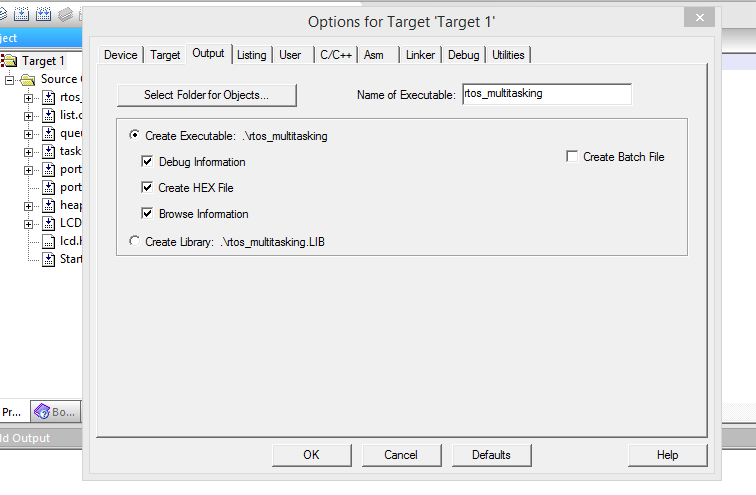
\includegraphics[width=10cm,height=6cm]{Capture.PNG}
\caption{Create HEX}
\end{figure}
\item Go to the c++ option on the same window. On that same page we will see a include paths option. Open that to include the files as shown in the image.
\begin{figure}[H]
\centering
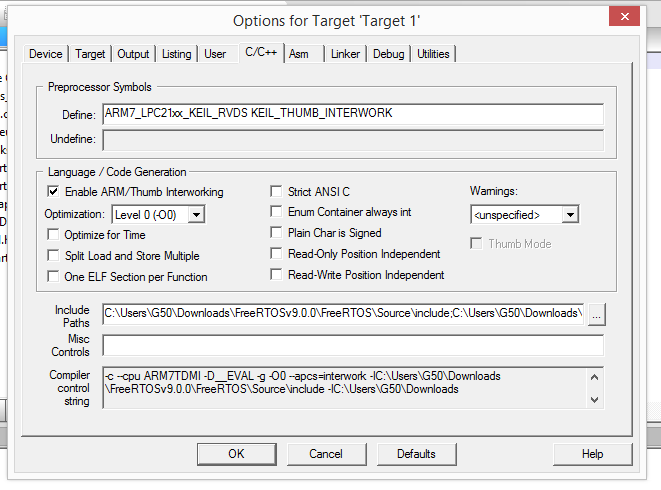
\includegraphics[width=10cm,height=6cm]{c++.PNG}
\caption{C++ configurations}
\end{figure}
\begin{figure}[H]
\centering
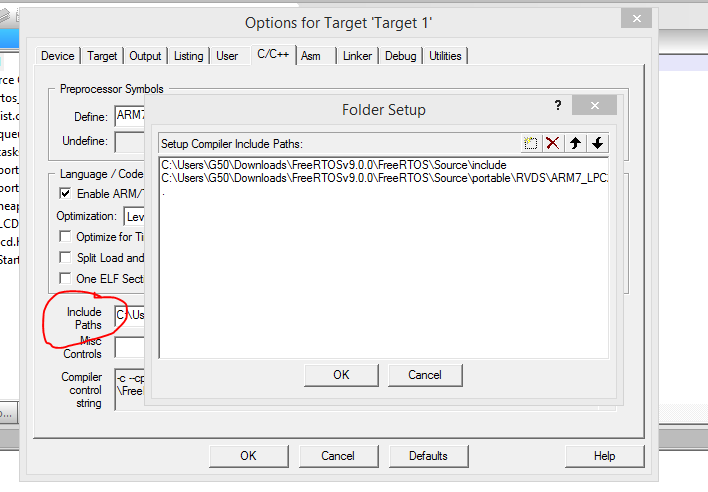
\includegraphics[width=10cm,height=6cm]{c++foldersetup.PNG}
\caption{C++ Folder Setup}
\end{figure}
\item After this go to the ASM page which is right next to the C++ page and again open the include paths page and include the following.
\begin{figure}[H]
\centering
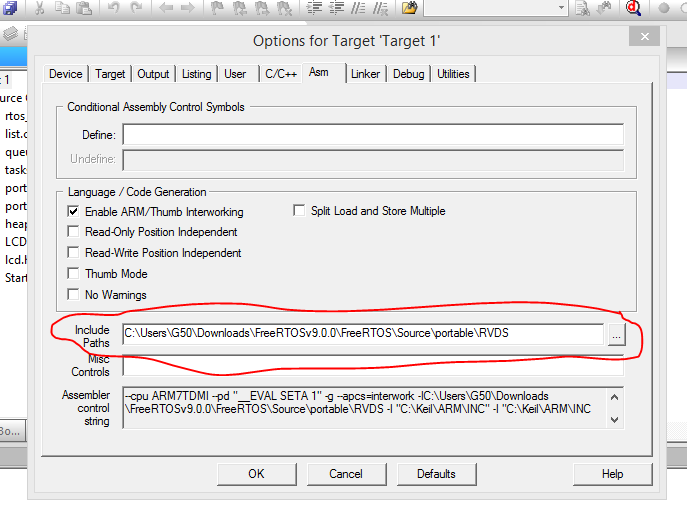
\includegraphics[width=10cm,height=6cm]{asm.PNG}
\caption{Include paths}
\end{figure}
\begin{figure}[H]
\centering
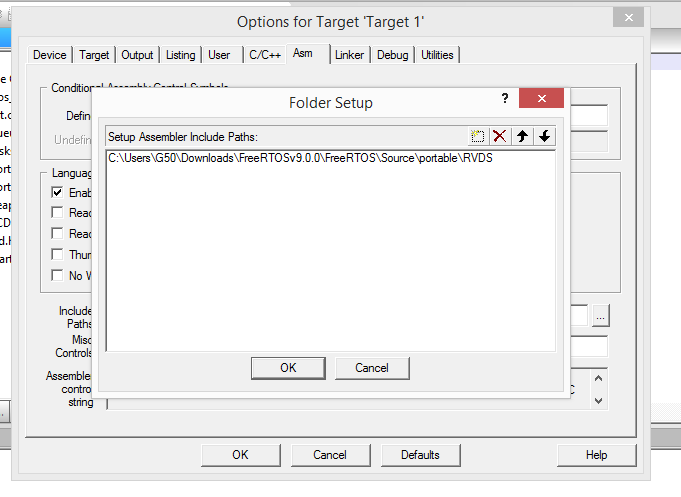
\includegraphics[width=10cm,height=6cm]{asmpath.PNG}
\caption{ASM Configurations}
\end{figure}

\item Go to the linker option and check the following settings.
\begin{figure}[H]
\centering
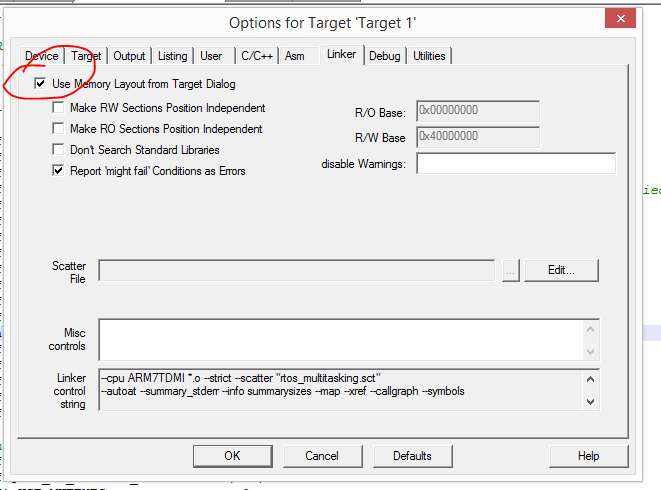
\includegraphics[width=10cm,height=6cm]{linker.PNG}
\caption{Include Files}
\end{figure}
Now lets begin including files to our project.
\item Firstly double click on the cource folder that is generated below the target folder.If it contains the 'startup.s' file then delete it.Include the new startup.s. This file is located in \\"FreeRTOSv9.0.0/FreeRTOS/Demo/ARM7LPC2129KeilRVDS" this folder.
\item Add the main.c file which contains our program.
\item Add the "tasks.c", "list.c" and "queue.c" from the source folder which is inside the FreeRTOSv9.0.0 folder which we downloaded.
\item Add the "FreeRTOS.h" and "freertosconfig.h" from include folder which is located inside the source folder.
\item Now go inside the portable folder inside the source folder and go to RVDS folder and open the ARMLPC21xx folder and add the "port.c" and "portASM.s".
\item And lastly inside the portable folder go to the "MemMang" folder and include the "heap2.c".
\item You can include the "LCD.c" from the experiments folder of FireBird V LPC2148 folder.\\
Your libraries should now consist of all these files.
\begin{figure}[H]
\centering
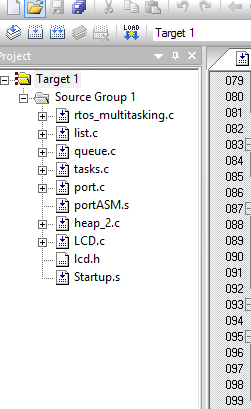
\includegraphics[width=7cm,height=10cm]{libraries.PNG}
\caption{LIBRARIES}
\end{figure}


\end{document}
